\section{Experimento 2}

\PARstart El segundo experimento que mostraremos fue realizado en los laboratorios del Departamento de Computación de FCEyN, más específicamente en el laboratorio 2.
La captura de paquetes duró una hora y se realizó sobre la red cableada del laboratorio, es decir, sobre Ethernet.
La modalidad fue desenchufar el cable Ethernet de la computadora 3 del laboratorio 2, y enchufándolo en nuestra propia computadora, de tal manera de poder capturar paquetes en modo promiscuo.

La captura de paquetes se realizó durante la tarde, mientras había aproximadamente 10 personas utilizando las computadoras de ese laboratorio. Las mediciones fueron realizadas con la autorización de uno de los administradores de la red, quien además ayudó a verificar las teorías que extrajimos de los paquetes. Veremos todo esto más adelante.

Antes de pasar a ver los resultados, una cosa que vale la pena decir es que, por como es la red de los laboratorios, al haber utilizado una computadora distinta de la de los laboratorios para realizar las mediciones, la red no nos asignó IP, es decir, no nos ``conectó'' de manera total a la red local. Sin embargo, esto no perjudicó en nada a las mediciones, y solo se vio reflejado en la fuente S.


\subsection{Resultados}

Primero analicemos la fuente S, que es la fuente de los paquetes unicast y broadcast. Como dijimos anteriormente, no teníamos dirección IP asignada. Esto sumado a que la red es switcheada, nos hace esperar que la cantidad de paquetes unicast que vamos a ver sea mucho más baja que lo normal. Esto, dicho en lenguaje de la Teoría de la Información, es que el símbolo que representa a los mensajes unicast tendrá una información más baja de la esperada.

Sin embargo, por como está configurada la red del laboratorio, sabemos que detrás de cada switch hay aproximadamente 4 o 5 computadoras, con lo cual podremos ver algunos paquetes unicast. Veamos qu\'e pasó.

\begin{figure}[H]
  \centering
  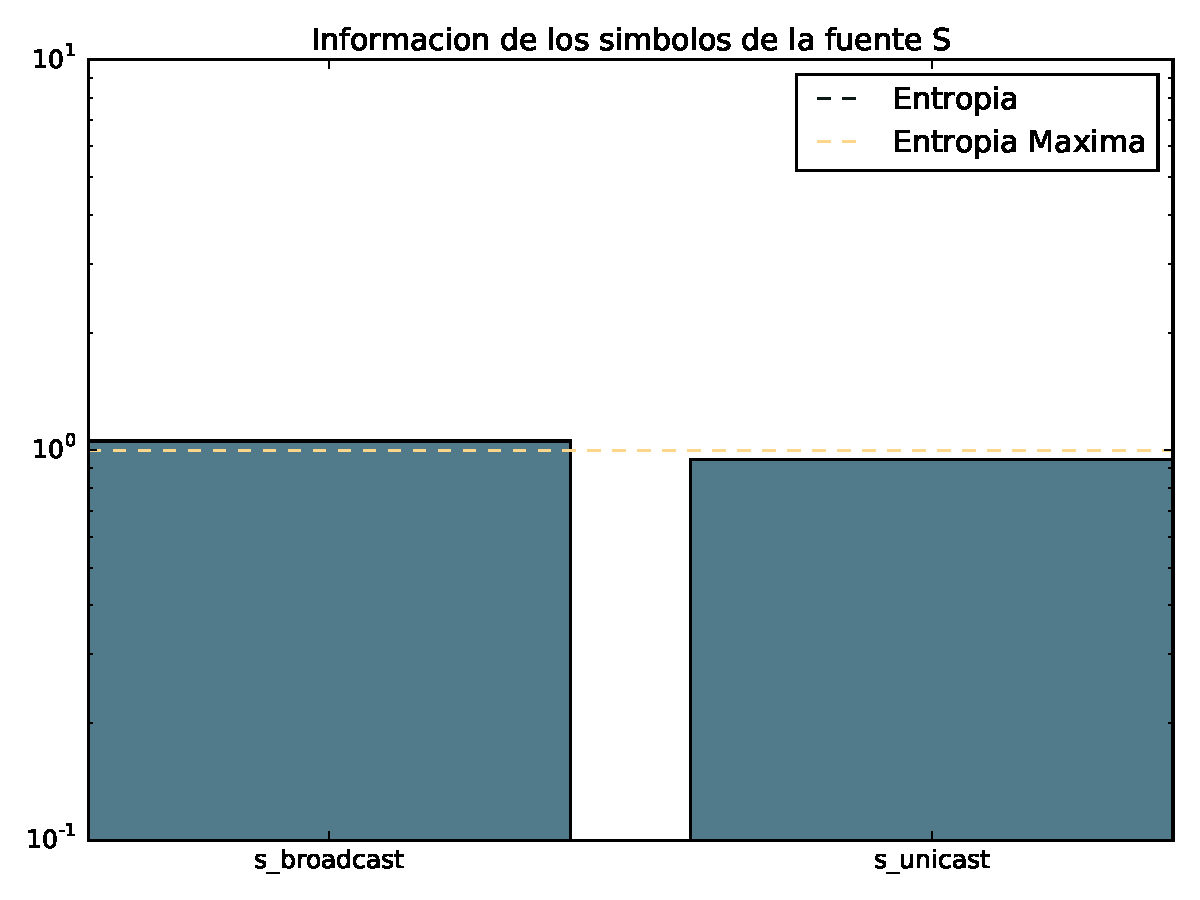
\includegraphics[width=8.5cm]{exp_labo/grafico1.pdf}
  \caption{\normalfont }
\end{figure}


Ahora pasemos a ver el diagrama de conectividad de la red, que nos permitirá saber más sobre cómo está configurada.

\begin{figure}[H]
  \centering
  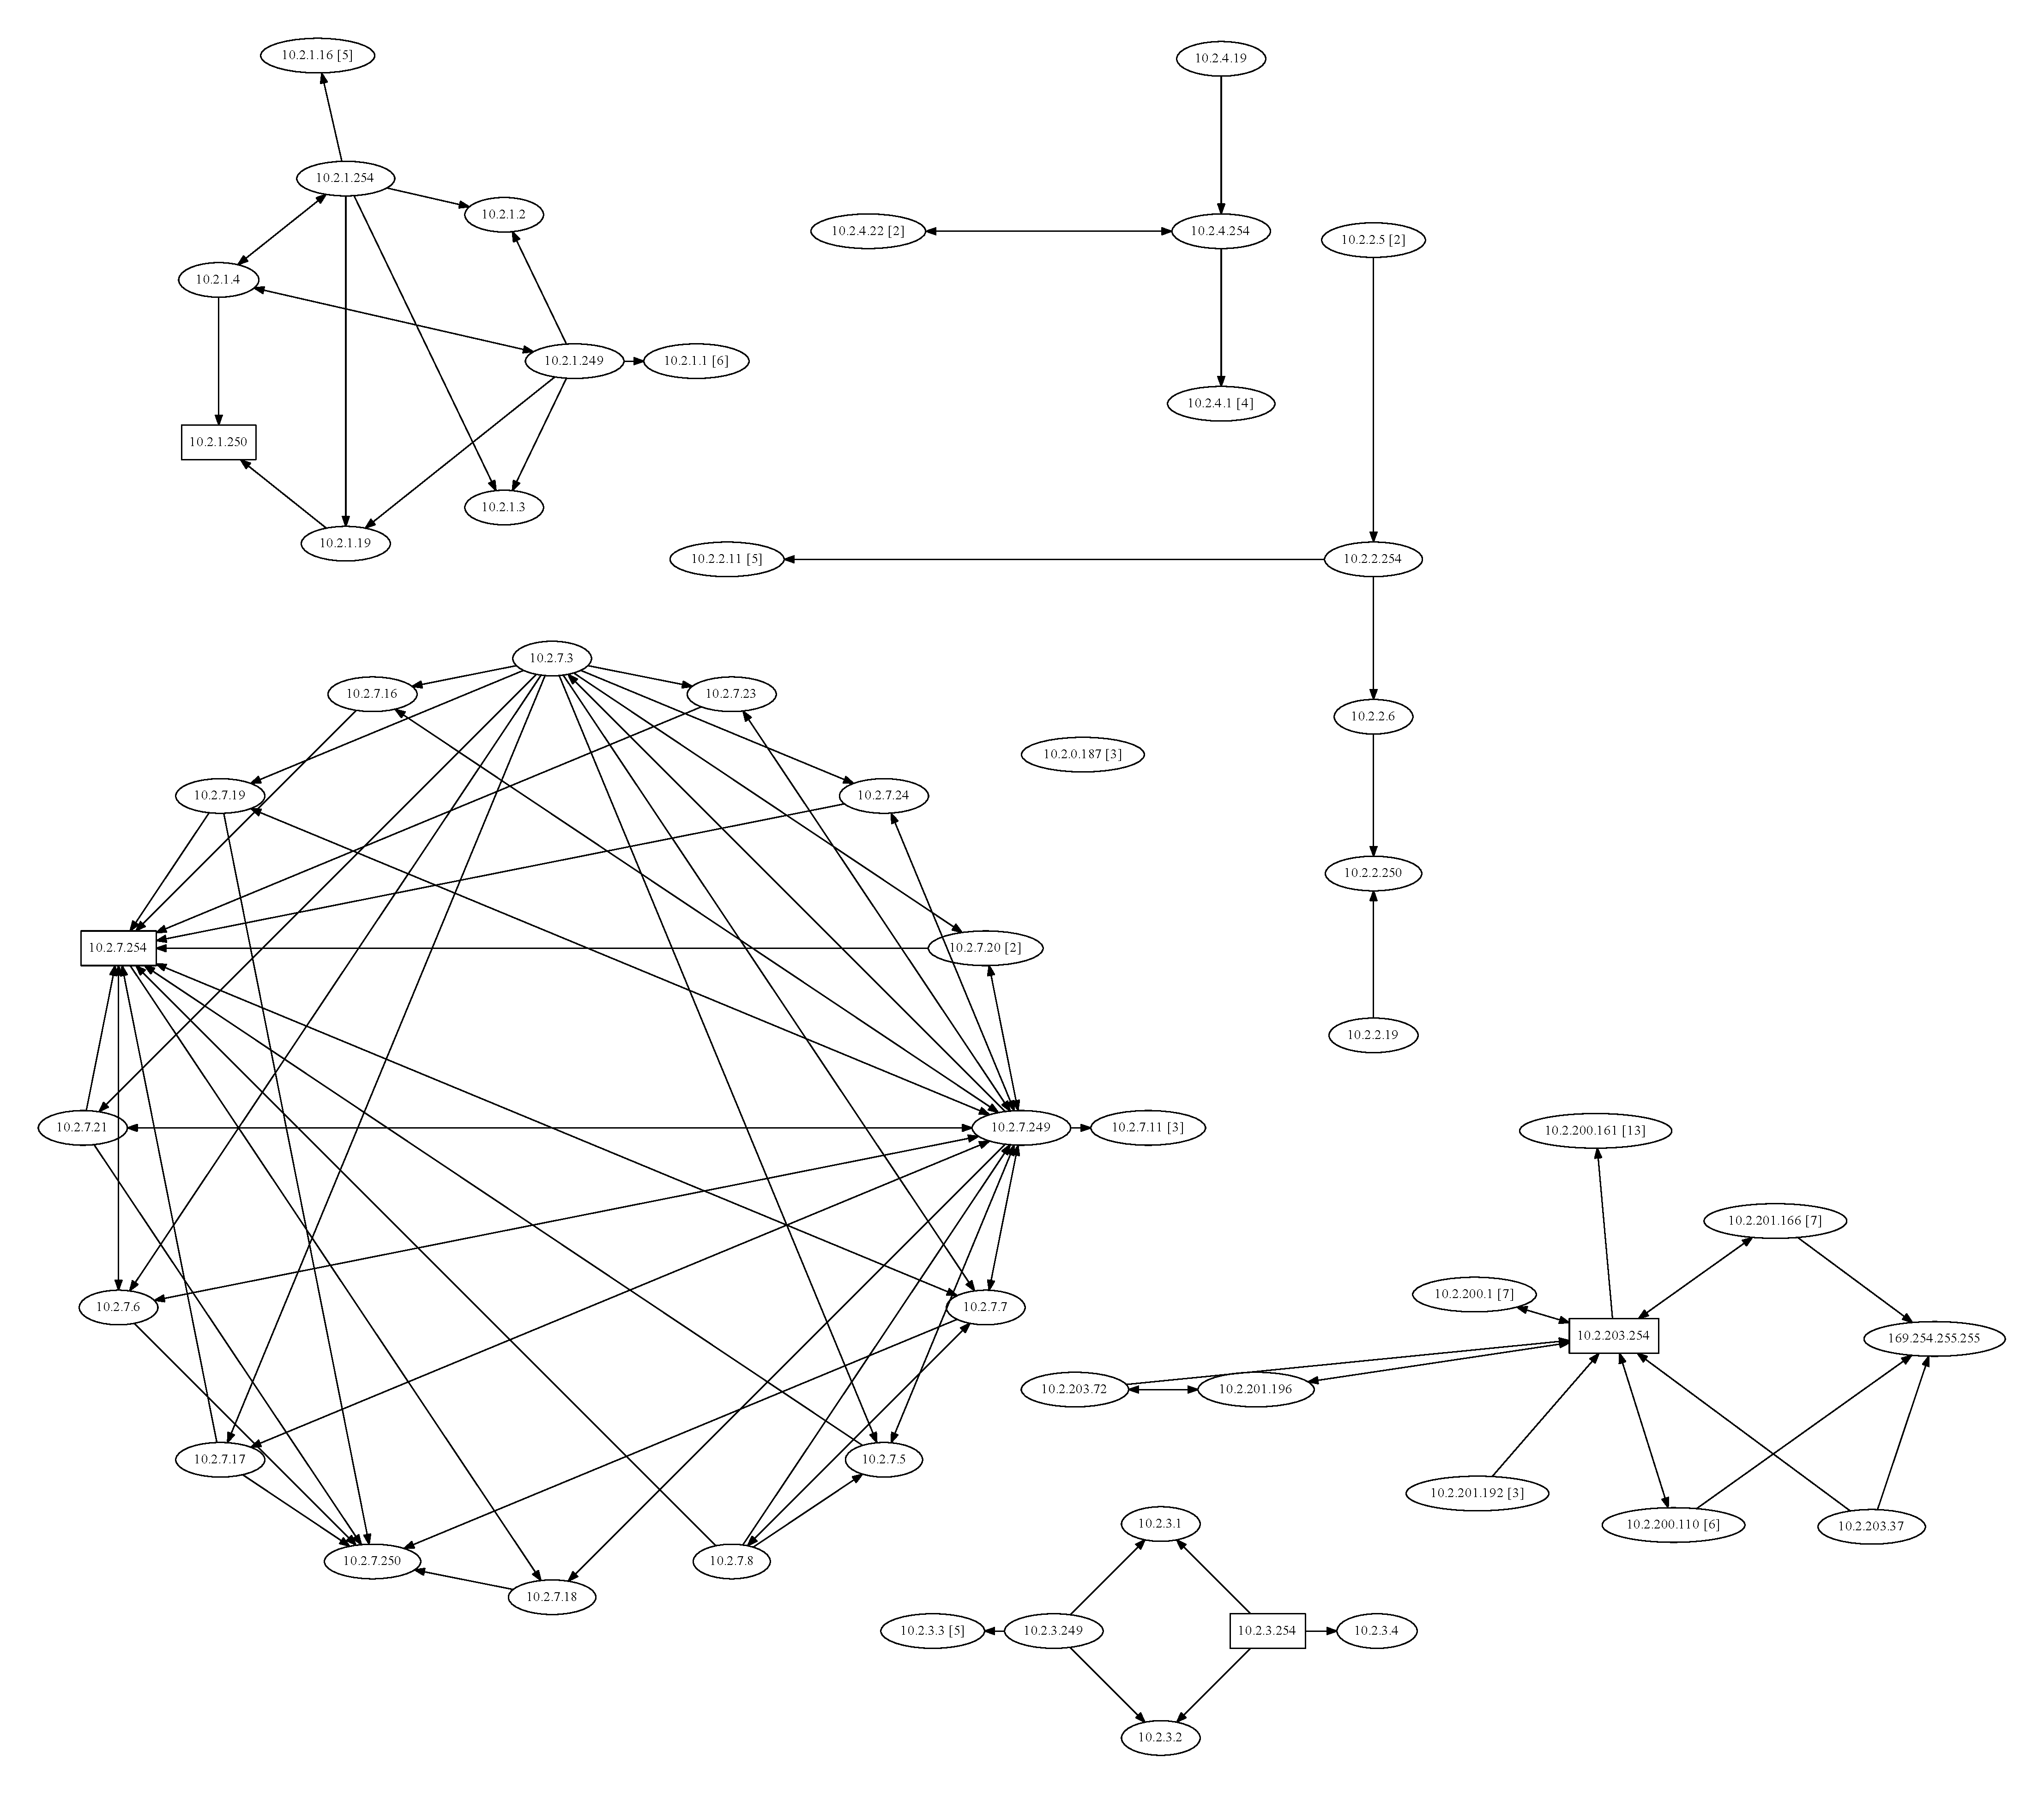
\includegraphics[width=8.5cm]{exp_labo/grafico2.pdf}
  \caption{  \normalfont Grafo de conectividad de la red, inferido de los paquetes who-has. Para ver con mayor detalle, se puede hacer zoom-in en el pdf. }
\end{figure}


\begin{figure}[H]
  \centering
  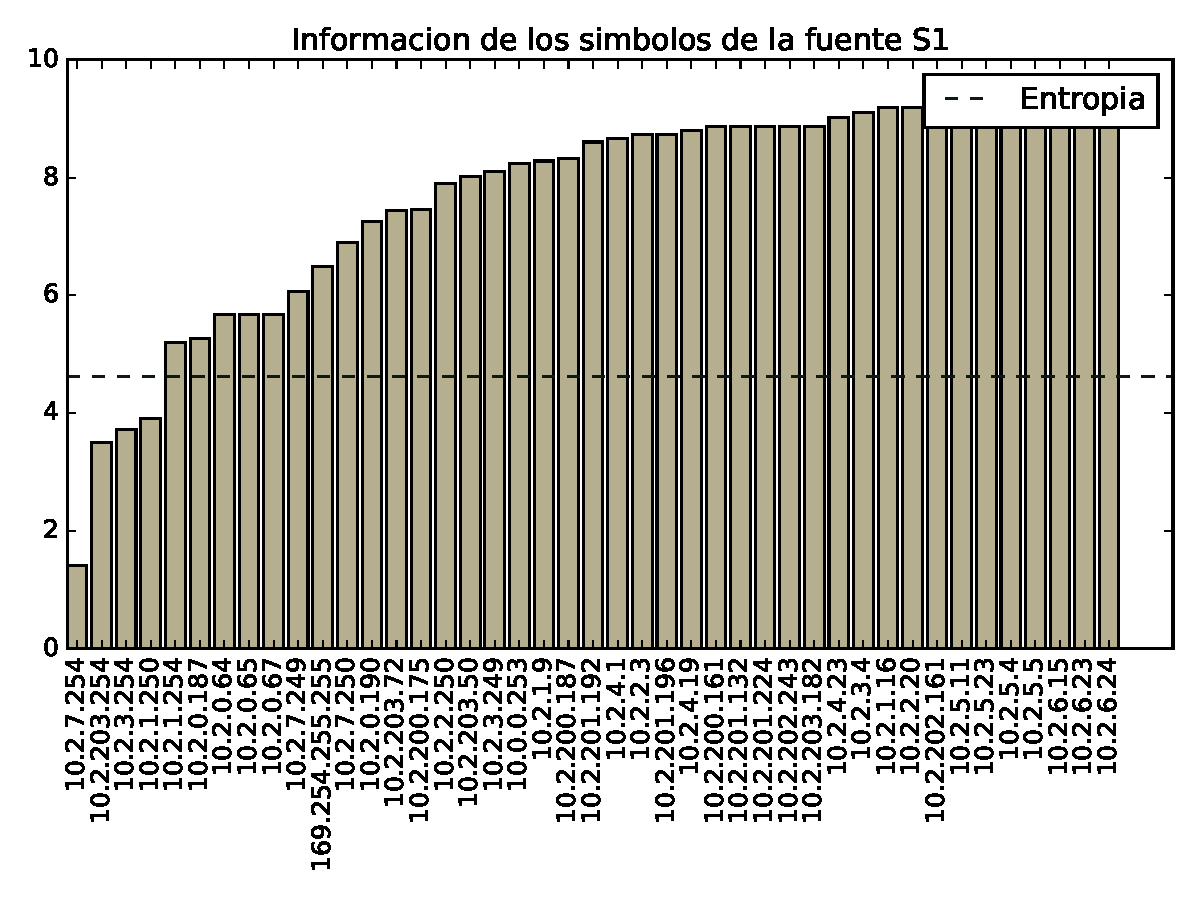
\includegraphics[width=8.5cm]{exp_labo/grafico3.pdf}
  \caption{ \normalfont Información de los símbolos de la fuente S1: solamente los nodos con menor información son representados.}
\end{figure}

\subsection{Discusión}

Para empezar, se confirma lo que dijimos sobre la fuente S: la información del símbolo de los paquetes unicast es mucho más alta de lo esperada e iguala casi a la de los paquetes broadcast. Esto provoca que la entropía sea muy cercana a la máxima. Desde el punto de vista de la probabilidad, esta fuente es menos predecible que la que vimos antes.

Además, si no hubi\'eramos sabido como estaba la configurada la red (que se ve a simple vista en los laboratorios), podríamos haber inferido que está fuertemente switcheada dada la información de estos símbolos.

Con lo cual, como dijimos al principio del trabajo, esta fuente nos permite saber, entre otras cosas, que tanta visibilidad tenemos de toda la red: a más visibilidad más paquetes unicast nos van a llegar, por lo tanto más baja va a ser la información del símbolo asociado.



Para continuar con el grafo de conectividad y la fuente S1, como vemos, hay muchos dispositivos en la red, contamos más de 100 dispositivos. Sin embargo, solo mostramos aquellos relevantes para la discusión. Esta cantidad nos dice que la red es muy compleja, y que salvo excepciones, seguramente tendrá alguna sub-estructuración interna, por ejemplo subnetting, y que por lo tanto será un desafío intentar comprenderla.


Yendo más a lo específico, se ve que hay un grafo muy similar a un grafo completo, que tiene un nodo distinguido con IP 10.2.7.254. Nuestra hipótesis será que este dispositivo es el router.
Además, todos los nodos de ese subgrafo tienen IPs de la forma 10.2.7.XXX.
Es decir, ese subgrafo representa la subred 10.2.7.0/24.
Por la cantidad y el detalle de nodos observados en esta subred, podemos inferir que es la red del laboratorio 2, donde capturamos los paquetes.
Sin embargo de ninguna manera podemos imaginarnos por que tantas de las computadoras se envían paquetes ARP unas a otras. Veremos la razón de esto más adelante.

Además, podemos observar que se repite el mismo patrón en distintos lugares, por lo que podemos asumir que son los distintos laboratorios. El patrón al que nos referimos es la IP de la pinta 10.2.n.XXX, donde n es el número de laboratorio y XXX es el número de host. Además, como antes, 10.2.n.254 suele ser el nodo distinguido, con lo cual podemos asumir que todos esos son los routers de cada laboratorio.

Hay otras 2 partes de la red que nos gustaría analizar. Primero, tres nodos de IP 10.2.0.XX, que lo único que hacen es mandar Gratitious ARP. Como vimos anteriormente, un Gratuitious ARP son paquetes broadcast que actúan como paquetes is-at, pero que nunca fueron pedidos.
Estos dispositivos actúan de manera anómala, pero como la red es muy compleja, podemos establecer como hipótesis que son dispositivos de control de la red.

Por último, podemos analizar la subred que se encuentra en la parte inferior izquierda de la figura. Como puede apreciarse, es bastante distinta al resto de las redes. 

Esta red sigue un patrón muy similar al que observamos anteriormente en la red Wi-Fi. Además, aparece la misma IP que había aparecido antes: 169.254.255.255. Por último, esta subred tiene un nodo distinguido terminado en 254: 10.2.203.254, así que nuestra hipótesis será que esta subred representa parte de la red Wi-Fi de los laboratorios de la facultad.


Luego de plantear todas nuestras hipótesis, nos pareció interesante consultar con un administrador de la red para saber que tan exactas fueron nuestras predicciones utilizando un modelo tan simple como usamos.

Resultó que nuestras predicciones fueron muy acertadas. Como predijimos, cada laboratorio se representa internamente con una subred. Estas subredes son las de la pinta 10.2.n.0/24. Además, los routers de cada labo son los de IP 10.2.n.254, como habíamos predicho.

Finalmente, el subgrafo que creíamos que se correspondía con la red Wi-Fi, efectivamente lo hacía. Según el administrador, esa subred corresponde a IPs de un pool dinámico de IPs, que se asignan en el rango de direcciones de 10.2.200.0 a 10.2.201.255 de forma dinámica cada vez que un dispositivo nuevo se conecta a la red. Dado que el Wi-Fi de los laboratorios está configurado con un pool dinamico de direcciones, y 10.2.203.254 es el router de la red. Quizás era un poco difícil
conocer toda esta información solamente con el grafo de conexiones, pero nos parece muy interesante contarlo de todas formas, porque es un patrón recurrente en redes Wi-Fi.

Además, nos aclaró que el hecho que las PCs de los laboratorios se manden paquetes unas a otras es esperado y tiene variadas causas. Primero, puede ser que dos usuarios est\'en usando un programa que use la red local, y entonces las computadoras se van a enviar paquetes ARP entre ellas. 
Otra cosa que sucede, es que las redes de los laboratorios tienen software de control y mantenimiento por temas de seguridad, y sobre todo para hacer que la red sea más fácil de mantener. Además es algo necesario para poder implementar el sistema conocido como Milagro, para poder conectarse a los laboratorios a trav\'es de ssh.

Por último, el administrador desconocía la razón por la cual había ciertos nodos que lo único que hacían era enviar Gratuitous ARP. Nos parece interesante plantear este interrogante como trabajo futuro.
